\section{Application-Specific Storage Stacks}
\label{sec:application-specifc-storage-stacks}

Building storage stacks from the ground up for a specific purpose results in
the best performance. For example, GFS~\cite{ghemawat:sosp03} and
HDFS~\cite{shvachko:msst10} were designed specifically to serve Map/Reduce and
Hadoop jobs, and use techniques like exposing data locality and relaxing POSIX
constraints to achieve application-specific I/O optimizations. Another example
is Boxwood~\cite{maccormick:osdi04}, which experimented with B-trees and chunk
stores as storage abstractions to simplify application building.
Alternatively, general-purpose storage stacks are built with the flexibility to
serve many applications by providing a variety of interfaces and tunable
parameters.  Unfortunately, managing competing forces in these systems is
difficult and users want more control from the general-purpose storage stacks
without going as far as building their storage system from the ground up.

To demonstrate a recent trend towards more application-specific storage systems
we examine the state of programmability in Ceph. Something of a storage Swiss
army knife, Ceph simultaneously supports file, block, and object interfaces on
a single cluster~\cite{ceph_contributors_ceph_2010}. Ceph's Reliable Autonomous
Distributed Object Storage (RADOS) system is a cluster of object storage
devices that provide Ceph with data durability and integrity using
replication, erasure-coding, and scrubbing~\cite{weil_rados_2007}. Ceph already
provides some degree of programmability; the object storage daemons support domain-specific
object interfaces that are implemented by composing existing low-level storage
interfaces that execute atomically. These interfaces are written in C++ and are
statically loaded into the system.

The Ceph community provides empirical evidence that developers are already
beginning to embrace programmable storage. Figure~\ref{fig:obj-int-dev-growth}
shows a dramatic growth in the production use of domain-specific interfaces in
the Ceph community since 2010. In that figure, classes are functional groupings
of methods on storage objects (e.g. remotely computing and caching the checksum
of an object extent).  What is most remarkable is that this trend contradicts
the notion that API changes are a burden for users.  Rather it appears that
gaps in existing interfaces are being addressed through ad-hoc approaches to
programmability. In fact, Table~\ref{table:objclasses} categorizes existing
interfaces and we clearly see a trend towards reusable services.

\begin{figure}[ht]
\centering
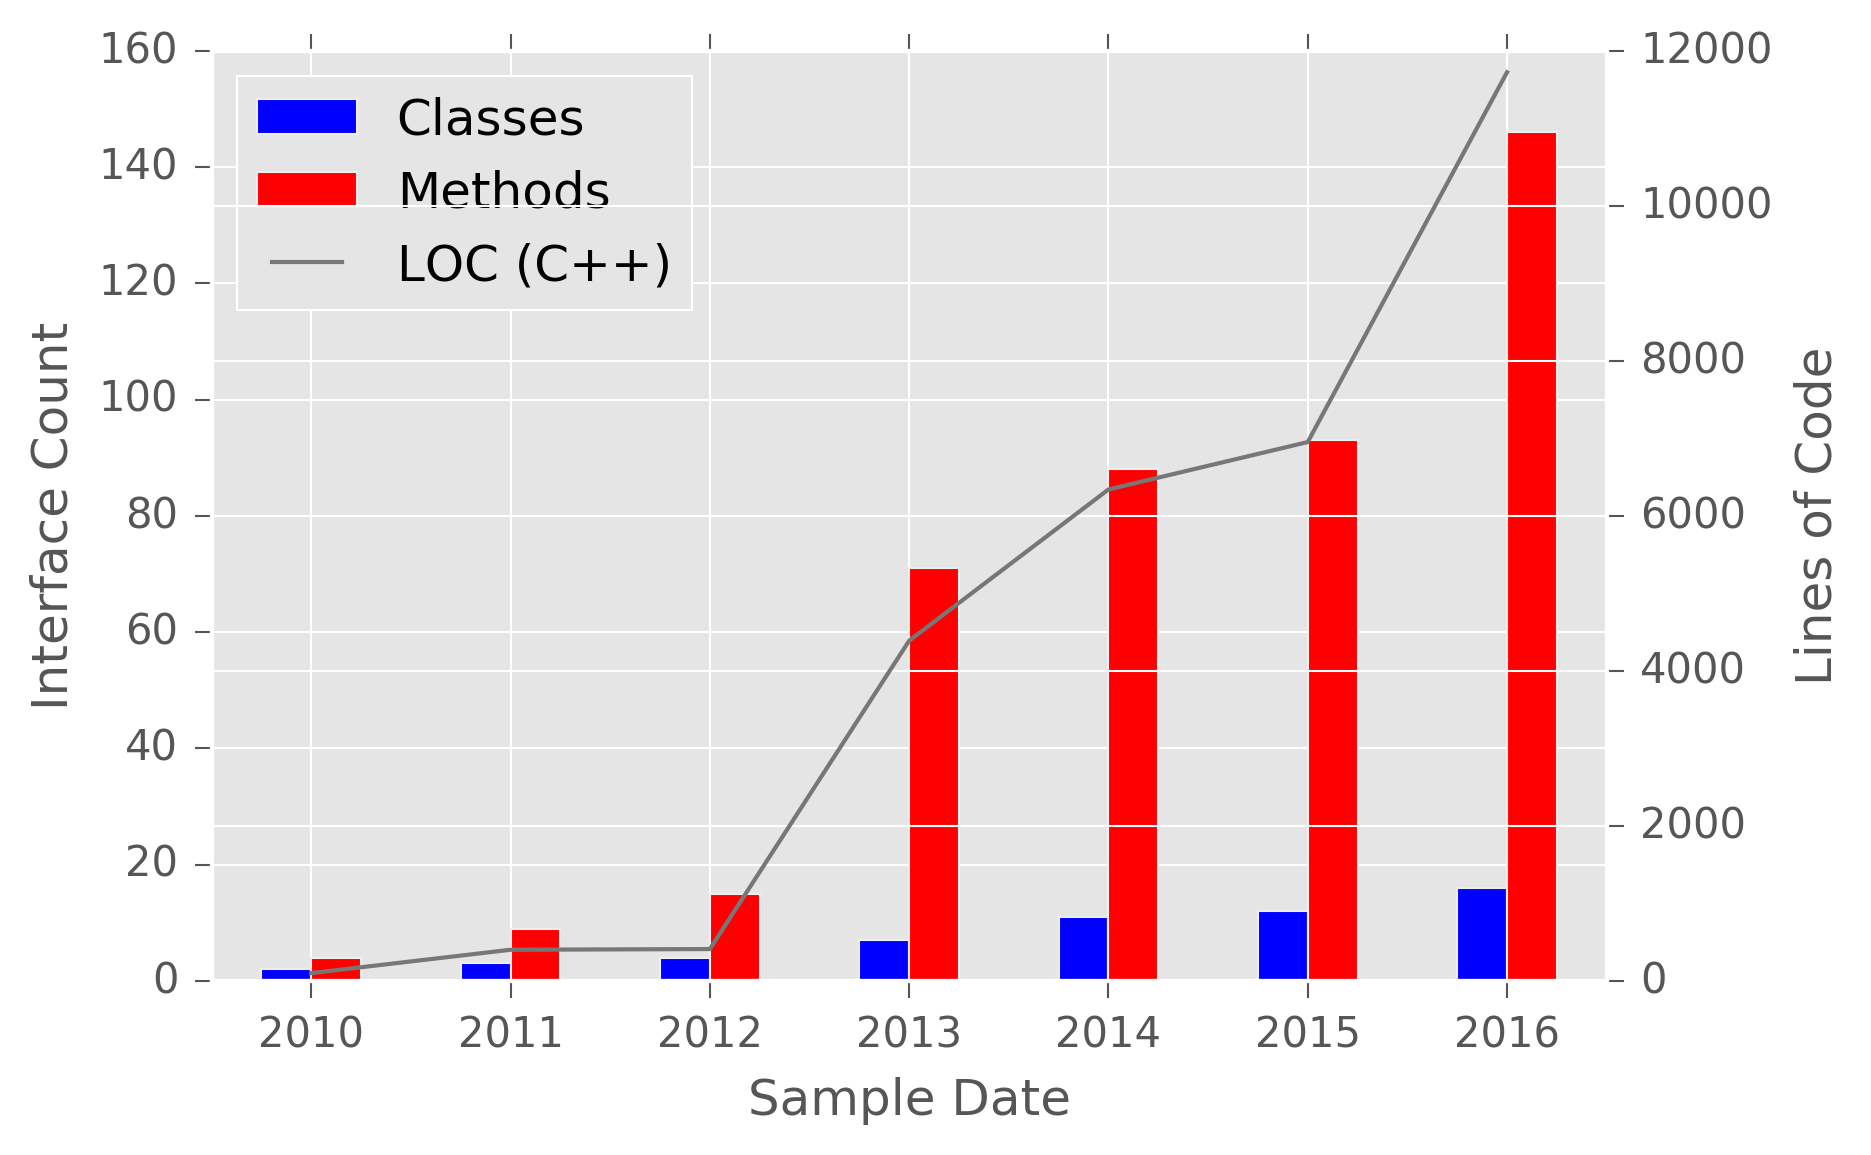
\includegraphics{figures/obj-int-dev-growth.png}
\caption{Since 2010, the growth in the number of co-designed object storage
interfaces in Ceph has been accelerating. This plot is the number of object
classes (a group of interfaces), and the total number of methods (the actual
API end-points).}
\label{fig:obj-int-dev-growth}
\end{figure}

\begin{table}[ht]
\centering
  \begin{tabular}{l|l|l}
    Category & Example & \# \\ \hline
    Logging  & Geographically distribute replicas & 11 \\ \hdashline
    Metadata & Snapshots in the block device OR  & \multirow{2}{*}{74} \\
    Management & Scan extents for file system repair & \\ \hdashline
    Locking  & Grants clients exclusive access & 6 \\ \hdashline
    Other & Garbage collection, reference counting  & 4\\
\end{tabular}
\caption{A variety of object storage classes exist to expose interfaces
    to applications. \# is the number of methods that implement these categories.
}
\label{table:objclasses}
\end{table}

The takeaway from Figure~\ref{fig:obj-int-dev-growth} is that programmers are
already trying to use programmability because their needs, whether they be
related to performance, availability, consistency, convenience, etc., are not
satisfied by the existing default set of interfaces. The popularity of the
custom object interface facility of Ceph could be due to a number of reasons,
such as the default algorithms/tunables of the storage system being
insufficient for the application's performance goals, programmers wanting to
exploit application-specific semantics, and/or programmers knowing how to
manage resources to improve performance. A solution based on
application-specific object interfaces is a way to work around the
traditionally rigid storage APIs because custom object interfaces give
programmers the ability to tell the storage system about their application: if
the application is CPU or I/O bound, if it has locality, if its size has the
potential to overload a single node, etc.  Programmers often know what the
problem is and how to solve it, but until the ability to modify object
interfaces, they had no way to express to the storage system how to handle
their data.

Our approach is to expose more of the commonly used, code-hardened subsystems
of the underlying storage system as interfaces. The intent is that these
interfaces, which can be as simple as a redirection to the persistent data
store or as complicated as a strongly consistent directory service, should be
used and re-used in many contexts to implement a wide range of services. By
making programmability a `feature', rather than a `hack' or `workaround', we
help standardize a development process that now is largely ad-hoc.
